\usetikzlibrary{angles}
\begin{center}
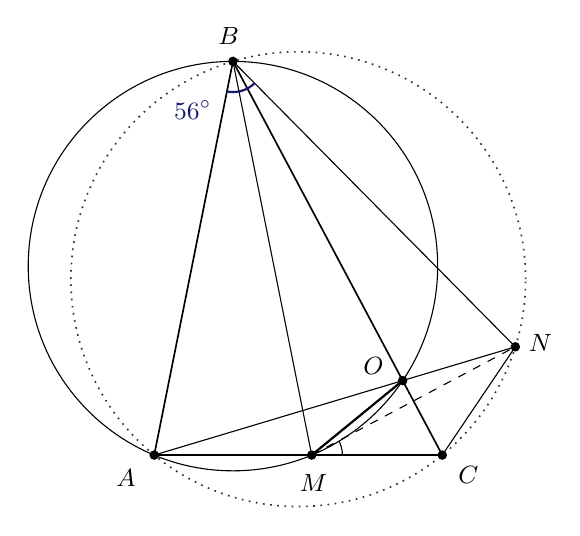
\begin{tikzpicture}[scale=1, font=\small]
    \providecolor{MidnightBlue}{cmyk}{0.98,0.13,0,0.43}
    \coordinate (A) at (0, 0);
    \path (A) ++(-0.36, -0.29) node[inner sep=0pt] {$A$};
    \coordinate (B) at (1, 5);
    \path (B) ++(-0.055, 0.32) node[inner sep=0pt] {$B$};
    \coordinate (M) at (2, 0);
    \path (M) ++(0.025, -0.35) node[inner sep=0pt] {$M$};
    \coordinate (C) at (3.65855, 0);
    \path (C) ++(0.33, -0.25) node[inner sep=0pt] {$C$};
    \coordinate (N) at (4.58599, 1.375);
    \path (N) ++(0.32, 0.05) node[inner sep=0pt] {$N$};
    \coordinate (O) at (3.1555, 0.9461);
    \path (O) ++(-0.37, 0.18) node[inner sep=0pt] {$O$};

    \draw[thin] (1, 2.4) circle (2.6);
    \draw[semithick, opacity=0.8, dotted] (1.82927, 2.23415) circle (2.8875);
    \draw[semithick] (A)--(B);
    \draw[semithick] (B)--(C);
    \draw[semithick] (C)--(A);
    \draw[thin] (A)--(N);
    \draw[thin] (B)--(M);
    \draw[thin] (B)--(N);
    \draw[thin] (N)--(C);
    \draw[thin, dashed] (M)--(N);
    \draw[thick] (M)--(O);
    \pic[draw=MidnightBlue, thick, angle radius=0.39cm] {angle=A--B--N};
    \node[inner sep=0pt, text=MidnightBlue] at (0.49, 4.38) {$56^{\circ}$};
    \pic[draw=black, angle radius=0.39cm] {angle=C--M--N};

    % Radius cetak titik tetap 1.5pt saat scale diubah.
    \pgfgettransformentries{\studioXX}{\studioYX}{\studioXY}{\studioYY}{\studioDX}{\studioDY}
    \pgfmathsetlengthmacro{\studioRadiusTitik}{1.5pt/veclen(\studioXX,\studioYX)}
    \foreach \s in {A,B,M,C,N,O}
        \filldraw (\s) circle (\studioRadiusTitik);
\end{tikzpicture}
\end{center}
